\chapter{Especificación de requisitos}

\noindent\fbox{
	\parbox{\textwidth}{
		En esta capítulo se tratarán de recoger todos los detalles que definan y limiten el funcionamiento de la aplicación.
	}
}

\section{Personas: ¿Quienes lo podrían usar?}

Para poder hacernos una idea de los posibles usos del Asistente de Voz se ha decidido crear una serie de personas ficticias que, para poder facilitar algún aspecto de su vida, puedan usar este producto.

El hecho de introducir personas para obtener requisitos viene a partir de que es un producto que desconocemos quién lo va a usar. No es un producto a medida mandado por alguien a quien podamos preguntarle por su visión de la aplicación final. Por ello, entra en juego este recurso. El uso de personas ficticias en desarrollo de software es una técnica que permite buscar cualquier problema que se pueda presentar si el concepto se llevara a producir, con tal de buscar soluciones o compromisos a asumir.

En las tablas de las siguientes páginas, podemos encontrar una información somera de estas personas:

\begin{itemize}
	\item \textbf{Irene Fernández}, una estudiante de Bachiller en una fase de exámenes finales antes de la Selectividad, donde acaba por planear su estudio y el tiempo que le queda para poder acabar el curso y entrar a su carrera vocacional en la Universidad.
	
	\item \textbf{Javier Pedrosa}, un funcionario que recientemente perdió parte de la visión por un accidente, entrando en una nueva fase de su vida donde la tecnología le ayuda a poder tener cierta autonomía.
\end{itemize}

Si bien estos casos pueden necesitar soluciones concretas, el objetivo con este proyecto es que si alguna función no se pudiera realizar en este momento, gracias a la modularidad cualquiera pudiera integrar alguna utilidad para suplir esas demandas.

\begin{table}[H]
	\centering
	\begin{tabular}{|l|l|l|} 
		\hline
		Nombre       & Irene Fernández & \multirow{4}{*}{
			\begin{minipage}[t]{0.4\textwidth}
				\begin{center}
					 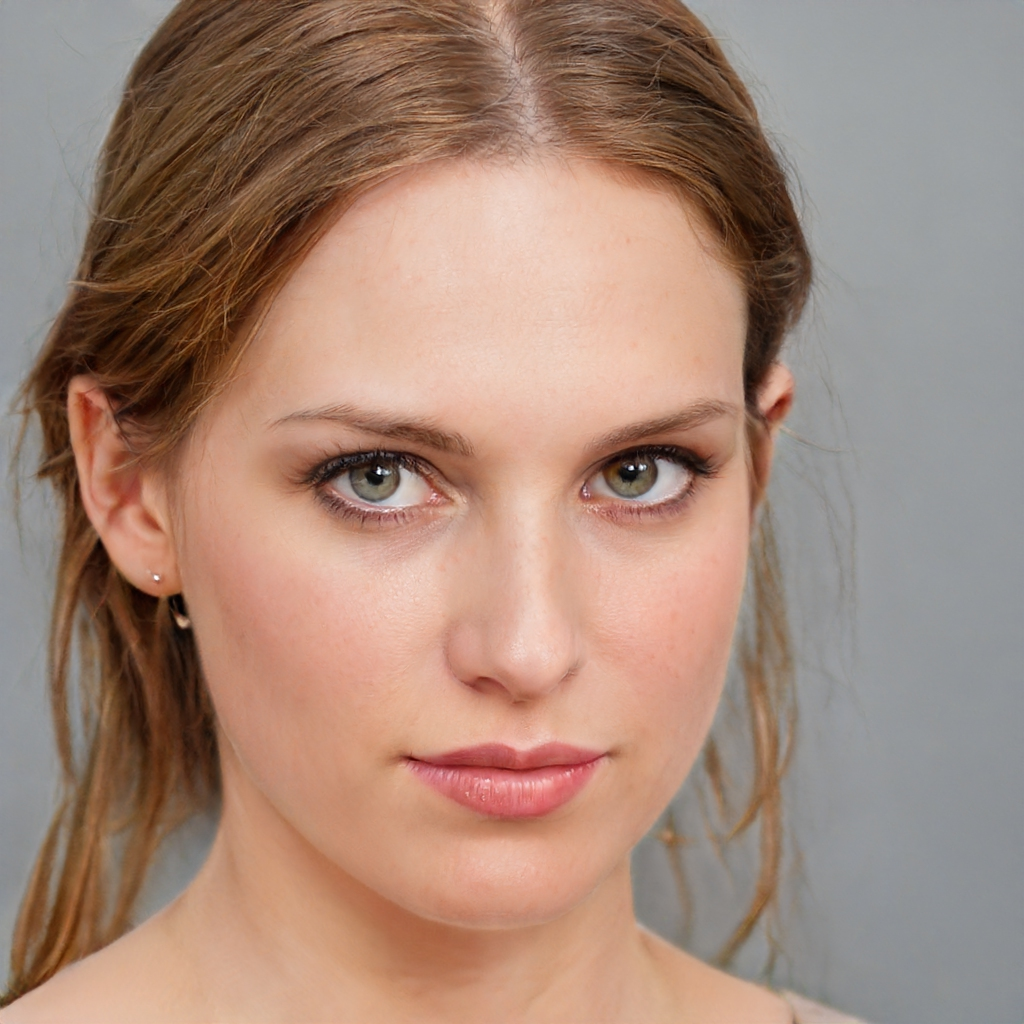
\includegraphics[height=3cm]{imagenes/Persona1.jpg}
				\end{center}
			\end{minipage}
			}                 \\ [2ex]
		\cline{1-2}
		Edad         & 19 &                                   \\ [2ex] 
		\cline{1-2}
		Género         & Femenino &                                   \\ [2ex]
		\cline{1-2}
		Educación    & Bachillerato Científico-Sanitario &                                   \\ [2ex] 
		\hline
		\multicolumn{3}{|l|}{{\cellcolor{lightblue}}\textbf{Contexto de uso}}               \\ 
		\hline
		Cuándo       & \multicolumn{2}{l|}{Tras las clases, antes de ponerse a estudiar}                \\ 
		\hline
		Dónde        & \multicolumn{2}{l|}{Ordenador portátil}                \\ 
		\hline
		\multicolumn{3}{|l|}{{\cellcolor{lightblue}}\textbf{Misión}}                        \\ 
		\hline
		Objetivo     & \multicolumn{2}{l|}{Tener una ayuda en el estudio}                \\ 
		\hline
		Expectativas & \multicolumn{2}{l|}{
			\begin{minipage} [t] {0.7\textwidth}
				\begin{itemize}
					\item Permitir hacer control del tiempo a través de contadores regresivos
					\item Permitir realizar cálculos sencillos
					\item Recordar tareas pendientes
				\end{itemize}
			\end{minipage}
		}                \\ 
		\hline
		\multicolumn{3}{|l|}{{\cellcolor{lightblue}}\textbf{Motivación}}                   \\ 
		\hline
		Urgencia     & \multicolumn{2}{l|}{
			\begin{minipage}[t]{0.7\textwidth}
				No le sería de mucha urgencia, ya que puede usar otras herramientas (Reloj/Cronómetro, Agenda, Calculadora...)
			\end{minipage}
		}                \\ 
		\hline
		Deseo        & \multicolumn{2}{l|}{
			\begin{minipage}[t]{0.7\textwidth}
				Siente que llevar tantas cosas para poder organizar su vida puede ser un tanto engorro, y centralizar sus utilidades en algo que lleve consigo como su portátil o su teléfono podría ahorrarle tantas molestias.
			\end{minipage}
		}                \\ 
		\hline
		\multicolumn{3}{|l|}{{\cellcolor{lightblue}}\textbf{Actitud ante la tecnología}}    \\ 
		\hline
		\multicolumn{3}{|l|}{
			\begin{minipage}[t]{\textwidth}
				Sabe manejar el ordenador en programas de ofimática como Word y Powerpoint; usa el navegador constantemente para ver sus redes sociales y buscar lo que necesite
			\end{minipage}
		}                              \\
		\hline
	\end{tabular}
	\caption[Ficha Persona 1]{Ficha de la Persona 1 (Irene Fernández). Imagen extraída de \cite{thispersondoesnotexist}}
\end{table}

\newpage

\begin{table}[H]
	\centering
	\begin{tabular}{|l|l|l|} 
		\hline
		Nombre       & Javier Pedrosa & \multirow{4}{*}{
			\begin{minipage}[t]{0.4\textwidth}
				\begin{center}
					
\includegraphics[height=3cm]{imagenes/Persona2.jpg}
				\end{center}
			\end{minipage}
		}                 \\ [2ex]
		\cline{1-2}
		Edad         & 46 &                                   \\ [2ex] 
		\cline{1-2}
		Género         & Masculino &                                   \\ [2ex]
		\cline{1-2}
		Profesión    & 
			\begin{minipage}[t]{0.3 \textwidth}
				Funcionario
			\end{minipage}
		 &                                   \\ [2ex] 
		\hline
		\multicolumn{3}{|l|}{{\cellcolor{lightblue}}\textbf{Contexto de uso}}               \\ 
		\hline
		Cuándo       & \multicolumn{2}{l|}{Al llegar a casa}                \\ 
		\hline
		Dónde        & \multicolumn{2}{l|}{Ordenador portátil y/o aparato dedicado}                \\ 
		\hline
		\multicolumn{3}{|l|}{{\cellcolor{lightblue}}\textbf{Misión}}                        \\ 
		\hline
		Objetivo     & \multicolumn{2}{l|}{Poder disfrutar de cierta independencia}                \\ 
		\hline
		Expectativas & \multicolumn{2}{l|}{
			\begin{minipage} [t] {0.7\textwidth}
				\begin{itemize}
					\item Permitir escuchar alguna información proveniente de Internet (Noticias, Tiempo...)
					\item Escuchar música, podcasts...
				\end{itemize}
			\end{minipage}
		}                \\ 
		\hline
		\multicolumn{3}{|l|}{{\cellcolor{lightblue}}\textbf{Motivación}}                   \\ 
		\hline
		Urgencia     & \multicolumn{2}{l|}{
			\begin{minipage}[t]{0.7\textwidth}
				No le sería de mucha urgencia, pero le encantaría tenerlo cuanto antes
			\end{minipage}
		}                \\ 
		\hline
		Deseo        & \multicolumn{2}{l|}{
			\begin{minipage}[t]{0.7\textwidth}
				Desde que perdió parcialmente la visión, no ha podido volver a dedicarse a pasiones como la literatura de forma fácil (por ejemplo, teniendo que esperar bastante tiempo para obtener audiolibros o libros adaptados a braille) o informarse en cualquier momento sin tener que pasar por el ordenador adaptado.
			\end{minipage}
		}                \\ 
		\hline
		\multicolumn{3}{|l|}{{\cellcolor{lightblue}}\textbf{Actitud ante la tecnología}}    \\ 
		\hline
		\multicolumn{3}{|l|}{
			\begin{minipage}[t]{\textwidth}
				Apenas usa el ordenador para alguna que otra gestión del trabajo.
			\end{minipage}
		}                              \\
		\hline
	\end{tabular}
	\caption[Ficha Persona 2]{Ficha de la Persona 2 (Javier Pedrosa). Imagen extraída de \cite{thispersondoesnotexist}}
\end{table}

\newpage

\section{Casos de uso: ¿Qué podrían hacer?}

Una vez pensado en posibles perfiles de uso, podríamos preguntarnos por alguna incidencia que pudiera solucionarse o facilitarse gracias al sistema resultante.

Los casos de uso en las metodologías ágiles nos permiten, a partir de las personas expuestas anteriormente, promover casos y analizarlos para encontrar posibles causísticas donde se pueda ver alguna inconformidad con el sistema resultante para tratar de paliarlo y prevenirlo en la fase de análisis.

\subsection{Caso 1: Irene y el calendario de exámenes}

Para nuestra primera persona podemos tener el siguiente caso:

`` \textit{5 de Abril de 2022. Se acerca la época de exámenes finales y poco a poco Irene va teniendo las fechas de estos. Viendo que es el momento de ponerse a prepararlos, apunta todos en su agenda, pero como en esta tiene además las tareas que ha de realizar, decide apuntar esos exámenes en el teléfono y en una hoja de calendario que tendrá que imprimir en la librería de al lado de su casa.}

\textit{Al llegar a casa, coge el teléfono y los va anotando. Además, descarga un PDF con el calendario del mes y llega a la tienda para imprimirlos. Al volver, también los anota, aunque con algo de prisa para ponerse a hacer las tareas que tenía que terminar para mañana. En el descuido los deja en un estante mal colocados y se caen al suelo mojado tras fregar la habitación, dejando la tinta borrosa.}

\textit{Al verlo, Irene se enfada un tanto por tener que volver a hacer el calendario.} ''

\textbf{¿Cómo se podría entonces solucionar este problema?} Podríamos aplicar el Asistente a través de una conversación donde se podría comunicar las fechas con tal de crear recordatorios o consultar a través de la voz si tiene algún evento en los próximos días.

Podríamos así tener una conversación para cada examen que quisiera introducir similar a:

\textit{
	\begin{itemize}
		\item \textbf{Irene}: Recuérdame que tengo examen de Historia de España el 22 de Abril.
		\item \textbf{Bot}: De acuerdo, el 22 de Abril te recordaré ``Examen de Historia de España''
	\end{itemize}
}

\subsection{Caso 2: Irene y la técnica Pomodoro}

Continuando con nuestra primera persona, podríamos darnos con otro caso en el que integrar el software podría servirle de ayuda.

`` \textit{15 de Abril de 2022. Una semana para el examen de Historia de España. Irene va a su cuarto con su reloj y prepara un temporizador de 25 minutos.}

\textit{Mientras estudia, se queda tan centrada que pasa al tiempo de descanso sin notar que el reloj ha vibrado. Cuando mira el reloj, se había pasado media hora más, así que se piensa hacer los 5 minutos de descanso en ese momento antes de activar el temporizador otra vez. Pero en ese caso tenía que estar pendiente del tiempo para no pasarse.} 

\textit{El día acabó siendo bastante fructífero y había preparado sus apuntes para poder seguir estudiando al día siguiente, pero fue un tanto molesto para ella ya que estar pendiente del reloj era un poco engorroso.}''

\textbf{¿Cómo se podría entonces solucionar este problema?} Podríamos aplicar el Asistente a través de dos cuentas atrás, una para la parte de estudio y otra para la parte de descanso, y pedir verbalmente que lo repita X veces, o que simplemente a través de pedir que ponga un contador Pomodoro se genere una conversación para configurar los tiempos y activarse automáticamente.

Podríamos así tener dos estilos de conversación:

La primera opción, que se repitiría tres veces:
\textit{
	\begin{itemize}
		\item \textbf{Irene}: Bot, ponme un contador de 25 minutos
		\item \textbf{Bot}: Contador en marcha
		\item \textbf{Bot}: *Suena alarma*
		\item \textbf{Irene}: Bot, ponme un contador de 5 minutos
		\item \textbf{Bot}: Contador en marcha
		\item \textbf{Bot}: *Suena alarma*
	\end{itemize}
}

La segunda opción, donde se configuraría una vez:
\textit{
	\begin{itemize}
		\item \textbf{Irene}: Bot, activa el contador Pomodoro
		\item \textbf{Bot}: Ok, ¿cuánto tiempo quieres ponerte a estudiar?
		\item \textbf{Irene}: 25 minutos
		\item \textbf{Bot}: De acuerdo. ¿Cuántos de descanso?
		\item \textbf{Irene}: 5 minutos
		\item \textbf{Bot}: Vale. ¿Y cuántas veces?
		\item \textbf{Irene}: Tres.
		\item \textbf{Bot}: De acuerdo. El tiempo de estudio comienza en 3,2,1... ¡Tiempo!
		\item \textbf{Bot}: (Tras 25 minutos) 3,2,1... ¡Es hora de un descanso!
		\item \textbf{Bot}: (Tras 5 minutos) 3,2,1... ¡Manos a la obra de nuevo!
		\item \textbf{Bot}: (Tras 25 minutos a la tercera vez) 3,2,1... *Alarma*
	\end{itemize}
}

\subsection{Caso 3: Javier y las noticias}

Para nuestra segunda persona, podríamos crear un caso en base a su condición especial:

``
\textit{Javier está sentado en el sofá escuchando la señal del canal de Noticias 24h cuando le llega un mensaje sobre una noticia de su pueblo. Quiere ir a leerlo pero el lector del teléfono se pone a leer partes de anuncios y se exaspera un tanto.}

\textit{Buscando otra alternativa, se pone en el ordenador con el visor Braille. Intentando abrir la noticia, debe teclearla letra a letra, incomodándose un poco. Finalmente, tras una pequeña odisea, logra digitar la noticia y enterarse de que un amigo de la infancia había salido en portada por un logro en el que había participado.}
''

\textbf{¿Cómo se podría entonces solucionar este problema?} Podríamos aplicar el Asistente a través de una conversación donde se podría poner a leer las noticias de un diario.

Podríamos así tener una conversación para cada examen que quisiera introducir similar a:

\textit{
	\begin{itemize}
		\item \textbf{Javier}: Bot, ¿podrías leerme las noticias del diario <Diario>?
		\item \textbf{Bot}: De acuerdo, aquí hay una noticia que dice así: ``Detenidos 2 vándalos que han pintado un tren del Metropolitano de Granada''. ¿Sigo leyendo?
		\item \textbf{Javier}: Siguiente.
		\item \textbf{Bot}: Vale, aquí hay otra noticia: ``Científicos de la UGR logran crear una memoria con materiales reciclados''. ¿Sigo leyendo?
		\item \textbf{Javier}: Si.
	\end{itemize}
}

En general, de los 3 casos podríamos sacar, sin entrar en las particularidades de cada caso:
\begin{enumerate}
	\item El sistema debe permitir una modularidad de forma que se puedan añadir nuevas funcionalidades sin necesidad de tocar todo el código principal.
	\item Habría que tener en cuenta el contexto donde se esté conversando, ya que no es lo mismo cuando le llega una orden durante una conversación que nada más activar la \textit{trigger word}
	\item Las respuestas deben sonar lo más claras y concisas posible.
	\item Las órdenes deberían tener cierta flexibilidad en su forma de expresarse, ya que para pedir, por ejemplo, que se inicie un temporizador, podríamos decir \textit{Activa un temporizador para dentro de X minutos} o \textit{Programa una cuenta atrás de X minutos}
\end{enumerate}


\begin{table}[H]
	\centering
	\begin{tabularx}{\textwidth}{|>{\columncolor{mintgreen}}c>{\columncolor{mintgreen}}X|}
		\hline
		
\includegraphics[width=30pt]{imagenes/Tarea_completada.png} & Con ello, cumplimos el Objetivo \textbf{O-DD 1.} (Diseñar personas y casos de uso en los que el software podría presentar algún problema con tal de buscar soluciones o limitaciones.) \\
		\hline
	\end{tabularx}
\end{table}

\section{Análisis competitivo}

Otra manera de encontrar posibles requisitos es observando a la competencia. Para ello podríamos analizar la funcionalidad de algunos de los competidores y sacar elementos comunes que podríamos traer en nuestro proyecto.

Para el análisis compararemos los siguientes proyectos, los cuales están mencionados en el capítulo 3 sobre el estado del arte:

\begin{itemize}
	\item \textbf{Amazon Alexa} \cite{alexa}, a través de un dispositivo Echo Dot previamente configurado para obtener señal de Internet y conectado a una aplicación en el teléfono a través de la cual se ha iniciado sesión con una cuenta de Amazon.
	\item \textbf{Microsoft Cortana} \cite{cortana}, a través de un ordenador con el Sistema Operativo Windows 10 instalado, y habiendo iniciado sesión previamente (pues es requerido por el programa)
	\item \textbf{Google Assistant} \cite{google-assistant}, a través de un teléfono móvil Android que se use a diario. Téngase en cuenta que para poder usar estos dispositivos se requiere tener una cuenta de Google.
\end{itemize}

Nótese que en el análisis queda fuera \textbf{Apple Siri} \cite{siri} ya que para ello requeriríamos de un dispositivo del ecosistema de Apple, y a fecha del análisis no se tenía en posesión de ningún dispositivo de la compañía.
\newpage

%\begin{xltabular}[H]
	\begin{xltabular}{\textwidth}{|c|X|X|X|}
		
		\hline \multicolumn{4}{|r|}{{Continúa en la siguiente página $>>$}} \\ \hline
		\endfoot
		
		\hline
		\endlastfoot
		
		\hline
		{\cellcolor{mintgreen}} \textbf{\textit{Propiedad}} & {\cellcolor{mintgreen}} \textbf{Alexa} & {\cellcolor{mintgreen}} \textbf{Cortana} & {\cellcolor{mintgreen}} \textbf{G-Assistant} \\
		\hline
		\textit{¿Dónde se puede usar?} & En dispositivos Echo y en la app Alexa & En ordenadores con Windows 10 y teléfonos Android y Apple & En teléfonos Android y en la web, además de dispositivos Google Home. \\
		\hline
		\begin{minipage}[t]{0.3\textwidth}
			\textit{¿Qué se necesita para empezar a usarlo?}
		\end{minipage} & Cuenta de Amazon y acceso a Internet & Acceso a Internet. Últimamente, cuenta de Microsoft. & Cuenta de GMail/Google y acceso a Internet.\\
	    \hline
	    \multirow{2}{*}{\begin{minipage}[t]{0.3\textwidth}
	    		\textit{¿Se puede añadir funcionalidades?¿Cómo?}
	    \end{minipage}}
	     & Se pueden programar \textit{skills} para distintos propósitos. Se puede descargar desde la app de Alexa. & Se podía, pero su creación ha quedado depreciada & Se permite a través del SDK de Google Actions. Se puede preguntar a la skill en concreto, aunque tiene su catálogo también para poder instalarlos\\
	     \cline{2-4}
         & \multicolumn{3}{c|}{\begin{minipage}[t]{0.6\textwidth}
        		En algunas skills habrá que tener en cuenta que se requiera iniciar sesión en alguna cuenta de terceros
        	\end{minipage}} \\
        \hline
        \begin{minipage}[t]{0.3\textwidth}
        	\textit{¿Cómo es el comportamiento en caso de que falle el Internet?}
        \end{minipage} & Avisa de que falta la conexión a Internet, pero reconoce la palabra clave & Al pulsar en el programa no contesta, pero informa de que no hay conexión & Al pulsar en el programa no contesta, pero informa de que no hay conexión\\
        \hline
        \begin{minipage}[t]{0.3\textwidth}
        	\textit{¿El asistente puede reconocer varias maneras de decir una misma frase?}
        \end{minipage} & Sigue ciertos patrones, y según la función permite cambiar la manera de expresar la orden o no & Tiene unas estructuras más fijas, no da mucho margen a expresar las órdenes de otra forma & Para funciones propias tiene una mayor variedad de patrones, pero para invocar las realizadas por otros se usa un patrón fijo \\ 
        \hline
        \begin{minipage}[t]{0.3\textwidth}
        	\textit{¿El asistente puede responder de varias maneras a una orden?}
        \end{minipage} & Para funciones que pueden cambiar en cualquier momento (por ej. Pedir la hora), suele tener una parte que no cambia, y según la función, añade ciertas frases. En otras órdenes, responde de forma aleatoria una respuesta de su repertorio. Si sólo tiene una, será esa la que se reproduzca & Responde de forma aleatoria una respuesta de su repertorio, o la única que tiene & Responde de forma aleatoria una respuesta de su repertorio, o la única que tiene \\ 
        \hline
	\caption{Análisis competitivo entre Alexa, Cortana y Google Assistant}
	\end{xltabular}
	
%\end{xltabular}

\begin{table}[H]
	\centering
	\begin{tabularx}{\textwidth}{|>{\columncolor{mintgreen}}c>{\columncolor{mintgreen}}X|}
		\hline
		
\includegraphics[width=30pt]{imagenes/Tarea_completada.png} & Con ello, cumplimos el Objetivo \textbf{O-IA 3.} (Analizar desde un punto de vista competitivo las prestaciones que ofrecen otras alternativas propietarias y libres (si las hay)) \\
		\hline
	\end{tabularx}
\end{table}

\section{La Ingeniería de Requisitos en acción}

\subsection{Requisitos funcionales}
A continuación se listarán aquellos requisitos que se requerirán para realizar el Asistente de Voz a un nivel de Producto Mínimo Viable. Esto no quiere decir que se puedan añadir más funcionalidades en un futuro. De haber más, se indicarán a lo largo del documento.

\begin{table}[H]
	\centering
	\begin{tabularx}{\textwidth}{|c|X|} 
		\hline
		\textbf{Nº de RF }          &  1 \\ 
		\hline
		\textbf{Nombre}         &  Hablar al Asistente \\ 
		\hline
		\textbf{Descripción}    &  Como usuario, quiero poder hablar con el programa para comunicarme con este \\ 
		\hline
		\textbf{Prioridad}      &  Alta  \\ 
		\hline
		\textbf{Entrada}        & Un sonido  \\ 
		\hline
		\textbf{Prerrequisitos} & Debe ser un audio hablado con la compresión que requiera las APIs que intervengan  \\ 
		\hline
		\textbf{Procesamiento}  &  Envía el audio para que el computador lo pueda entender \\ 
		\hline
		\textbf{Postcondición}  &  - \\
		\hline
	\end{tabularx}
	\caption{Descripción del Requisito Funcional 1: Hablar al Asistente}
\end{table}

\begin{table}[H]
	\centering
	\begin{tabularx}{\textwidth}{|c|X|} 
		\hline
		\textbf{Nº de RF }          &  2 \\ 
		\hline
		\textbf{Nombre}         &  Escuchar una respuesta del Asistente \\ 
		\hline
		\textbf{Descripción}    &  Como usuario, quiero poder escuchar la respuesta del programa para comunicarme con este \\ 
		\hline
		\textbf{Prioridad}      &  Alta  \\ 
		\hline
		\textbf{Entrada}        & Un sonido  \\ 
		\hline
		\textbf{Prerrequisitos} & La respuesta ha debido ser generada para poder pronunciarla \\ 
		\hline
		\textbf{Procesamiento}  &  Se generará un audio leyendo la respuesta conforme a los requisitos de la API que se use para reproducir el sonido. \\ 
		\hline
		\textbf{Postcondición}  &  - \\
		\hline
	\end{tabularx}
	\caption{Descripción del Requisito Funcional 2: Escuchar al Asistente}
\end{table}

\begin{table}[H]
	\centering
	\begin{tabularx}{\textwidth}{|c|X|} 
		\hline
		\textbf{Nº de RF }          &  3 \\ 
		\hline
		\textbf{Nombre}         &  Sintetizar la voz de una pregunta \\ 
		\hline
		\textbf{Descripción}    &  Como sistema, quiero poder leer la pregunta para comunicarme con el usuario \\ 
		\hline
		\textbf{Prioridad}      &  Alta  \\ 
		\hline
		\textbf{Entrada}        & Un sonido grabado  \\ 
		\hline
		\textbf{Prerrequisitos} & Debe ser un audio hablado con la compresión que requiera las APIs que intervengan \\ 
		\hline
		\textbf{Procesamiento}  &  A través de un algoritmo de Speech Recognition, convertir el audio en un texto \\ 
		\hline
		\textbf{Postcondición}  &  - \\
		\hline
	\end{tabularx}
	\caption{Descripción del Requisito Funcional 3: Sintetizar la voz de una pregunta.}
	\vspace{0.5cm}
	\centering
	\begin{tabularx}{\textwidth}{|c|X|} 
		\hline
		\textbf{Nº de RF }          &  4 \\ 
		\hline
		\textbf{Nombre}         &  Generar un audio con la respuesta \\ 
		\hline
		\textbf{Descripción}    &  Como sistema, quiero poder hablar la respuesta del programa para comunicarme con el usuario \\ 
		\hline
		\textbf{Prioridad}      &  Alta  \\ 
		\hline
		\textbf{Entrada}        & Una cadena de texto con la respuesta  \\ 
		\hline
		\textbf{Prerrequisitos} & - \\ 
		\hline
		\textbf{Procesamiento}  &  A través de un algoritmo de Text-To-Speech, convertir el texto en un audio \\ 
		\hline
		\textbf{Postcondición}  &  - \\
		\hline
	\end{tabularx}
	\caption{Descripción del Requisito Funcional 4: Generar un audio con la respuesta.}
	\vspace{0.5cm}
	\centering
	\begin{tabularx}{\textwidth}{|c|X|} 
		\hline
		\textbf{Nº de RF }          &  5 \\ 
		\hline
		\textbf{Nombre}         &  Relacionar una pregunta con una respuesta  \\ 
		\hline
		\textbf{Descripción}    &  Como sistema, quiero procesar la pregunta para poder ofrecer una respuesta \\ 
		\hline
		\textbf{Prioridad}      &  Alta  \\ 
		\hline
		\textbf{Entrada}        & Una cadena de texto con la respuesta  \\ 
		\hline
		\textbf{Prerrequisitos} & - \\ 
		\hline
		\textbf{Procesamiento}  &  Buscará a través de un patrón o similar una respuesta a la petición del usuario \\ 
		\hline
		\textbf{Postcondición}  &  - \\
		\hline
	\end{tabularx}
	\caption{Descripción del Requisito Funcional 5: Relacionar una pregunta con una respuesta.}
\end{table}


\begin{table}[H]
	\centering
	\begin{tabularx}{\textwidth}{|c|X|} 
		\hline
		\textbf{Nº de RF }          &  6 \\ 
		\hline
		\textbf{Nombre}         &  Avisar que no se puede conectar a Internet  \\ 
		\hline
		\textbf{Descripción}    &  Como sistema, quiero comunicar que no se ha podido conectar a Internet para que el usuario trate de arreglar la incidencia \\ 
		\hline
		\textbf{Prioridad}      &  Media  \\ 
		\hline
		\textbf{Entrada}        & - \\ 
		\hline
		\textbf{Prerrequisitos} & Se ha tenido que generar una pregunta previa que requiriese usar servicios en línea  \\ 
		\hline
		\textbf{Procesamiento}  &  Generará un audio para avisar que no se puede conectar \\ 
		\hline
		\textbf{Postcondición}  &  - \\
		\hline
	\end{tabularx}
	\caption{Descripción del Requisito Funcional 6: Avisar que no se puede conectar a Internet}
\end{table}

\begin{table}[H]
	\centering
	\begin{tabularx}{\textwidth}{|c|X|} 
		\hline
		\textbf{Nº de RF }          &  7 \\ 
		\hline
		\textbf{Nombre}         &  Responder que se desconoce la respuesta  \\ 
		\hline
		\textbf{Descripción}    &  Como sistema, quiero poder comunicar que no sé la respuesta a la pregunta para poder avisar al usuario \\ 
		\hline
		\textbf{Prioridad}      &  Media  \\ 
		\hline
		\textbf{Entrada}        & -  \\ 
		\hline
		\textbf{Prerrequisitos} & La pregunta dicha anteriormente no coincide con algún patrón o tipo de pregunta \\ 
		\hline
		\textbf{Procesamiento}  &  Generará un audio para responder al usuario \\ 
		\hline
		\textbf{Postcondición}  &  - \\
		\hline
	\end{tabularx}
	\caption{Descripción del Requisito Funcional 7: Responder que se desconoce la respuesta}
\end{table}

\subsection{Requisitos no funcionales}

\begin{enumerate}[\textbf{RNF-} 1.]
	\item \textbf{Usabilidad y legibilidad del código:} Debido a que va a ser un proyecto que luego se publicará y que además da pie a que otras personas colaboren en él, sería conveniente que el código sea lo más claro y conciso posible. Por tanto:
	\begin{itemize}
		\item Se realizará una \textbf{codificación modular}, de forma que los cambios estén lo más localizados posible y que no se requieran hacer muchos de ellos.
		\item El código deberá seguir los estándares y convenios de codificación del lenguaje \textbf{Python}. Para comprobarlo, usaremos como linter \textbf{PyLint} \cite{pylint}, ya que nos aconsejará y advertirá tanto de posibles errores lógicos como de código que haya que refactorizar para seguir esos estándares.
	\end{itemize}

	\item \textbf{Implementación:} Para realizar el proyecto, haremos uso de varias tecnologías. Principalmente, requeriremos:
		\begin{itemize}
			\item Como lenguaje de programación principal se usará una versión >=3.5 de \textbf{Python}.
			\item Se usarán APIs y Frameworks de Reconocimiento de Voz y de Text-to-Speech que posean licencias de \textbf{Software Libre} (GPL/LGPL/AGPL) o de \textbf{Código Abierto} (Licencia Apache/Mozilla/BSD).
			\item De la misma manera, aquellos Frameworks que persigan la relación entre las preguntas o peticiones del usuario y las respuestas del sistema deberán seguir esas mismas condiciones.
			\item En consecuencia, la versión de Python a utilizar deberá ser la última que soporten todas sus dependencias.
		\end{itemize}
	
	\item \textbf{Rendimiento}: Al ser un sistema que requiere una interacción con el usuario lo más fluida posible, tendremos que regir alguna restricción:
	\begin{itemize}
		\item El tiempo entre la pregunta y la respuesta no debería exceder de los 5 segundos.
	\end{itemize}

	\item \textbf{Información a utilizar}: Al ser un sistema que interactúa con el usuario, recogerá algunos datos sensibles como nombre, IP del dispositivo donde está instalado o la propia voz. Por tanto:
	\begin{itemize}
		\item Los datos que se usen para personalizar la experiencia no deberán ser enviados, a no ser que se requiera alguna conexión a Internet, en cuyo caso se daría sólo lo necesario (por ejemplo, si se registra un lugar para consultar el tiempo, sólo se debería enviar una petición para consultar esa información para ese lugar).
		\item El \textbf{tratamiento de la voz}, de ser posible, se realizará \textbf{en el propio dispositivo}.
		\item Si se requiriera enviar alguna información sensible más allá de lo contemplado, debería de al menos \textbf{notificarse} una vez al usuario (por ejemplo, en la configuración inicial o en la documentación).
	\end{itemize}
.
	\item \textbf{Ámbito legal}: Al ser un sistema que usa ciertas dependencias con licencias, sería necesario regularizar la situación con el siguiente requisito:
	\begin{itemize}
		\item La licencia del proyecto resultante deberá ser \textbf{compatible} con todas las dependencias utilizadas en este.
	\end{itemize}

	\item \textbf{Sistema}: El proyecto resultante debe poder ejecutarse en al menos algún dispositivo. Por tanto, las \textbf{características} del sistema a utilizar serían:
	\begin{itemize}
		\item Con \textbf{entrada y salida de audio}, bien soldado o cableado, bien a través de conectores (como Jack)
		\item Capaz de \textbf{ejecutar} la versión de \textbf{Python} y las dependencias asociadas
	\end{itemize}

	De cara al desarrollo usaremos dos dispositivos para poder probarlo:
	\begin{itemize}
		\item El \textbf{portátil} donde se desarrollará el proyecto.
		\item Una \textbf{Raspberry Pi 3B}, que tratará de emular a los dispositivos dedicados vistos en el Análisis Competitivo.
	\end{itemize}
	Estos usarán una distribución de \textbf{Linux} (\textit{Kubuntu 20.04} en el caso del portátil y \textit{Raspberry Pi OS} en el caso del dispositivo homónimo) siguiendo los requisitos de Implementación.
\end{enumerate}
 